%
% $RCSfile: template_method.tex,v $
%
% Copyright (c) 2004. Christian Heller. All rights reserved.
%
% No copying, altering, distribution or any other actions concerning this
% document, except after explicit permission by the author!
% At some later point in time, this document is planned to be put under
% the GNU FDL license. For now, _everything_ is _restricted_ by the author.
%
% http://www.cybop.net
% - Cybernetics Oriented Programming -
%
% http://www.resmedicinae.org
% - Information in Medicine -
%
% @author Christian Heller <christian.heller@tuxtax.de>
%

\paragraph{Template Method}
\label{template_method_heading}

The \emph{Template Method} pattern \cite{gamma1995}, also called
\emph{Hook Method}, is an abstract definition of the \emph{Skeleton} of an
algorithm. The implementation of one or more steps of that algorithm is
delegated to a sub class (figure \ref{templatemethod_figure}).

\begin{figure}[ht]
    \begin{center}
        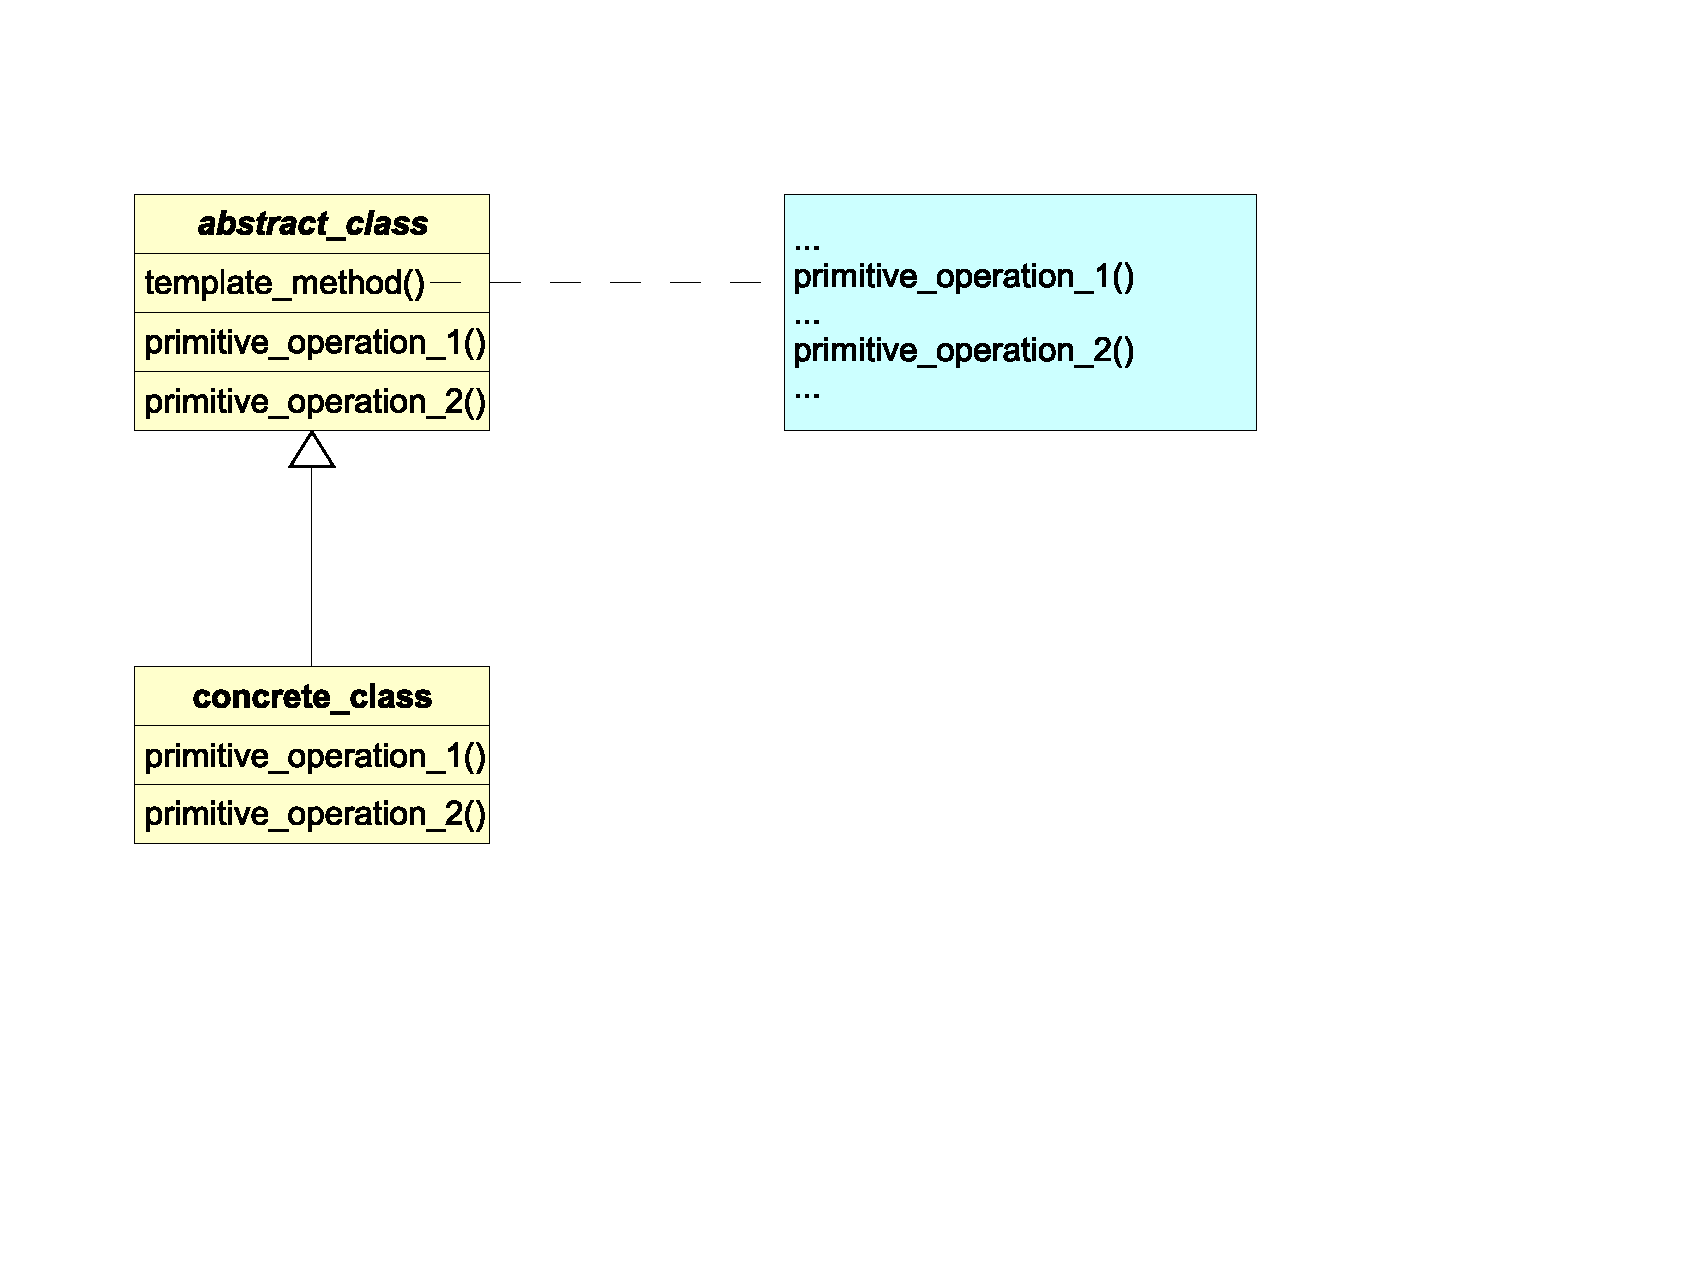
\includegraphics[scale=0.3]{vector/templatemethod.eps}
        \caption{Template Method Pattern}
        \label{templatemethod_figure}
    \end{center}
\end{figure}
